% The use of oneside here is a temporary hack; \marginpar entries
% don't show up on odd pages of PDF output without it.  Sigh.
%
%
%
%
\documentclass[oneside]{book}
\usepackage{enumerate}
\usepackage{algorithmic}
\usepackage{fullpage}
\usepackage{makeidx}
\usepackage{ifpdf}
\usepackage[pdftex]{graphicx}
\usepackage{pslatex}
\usepackage{fancyvrb}
\usepackage{float}
\usepackage{syntonly}
\usepackage{amsmath}  % for Mathmatic 
\usepackage{multirow} % for tables and tabular
\usepackage{shorttoc}
\floatstyle{ruled}
\newfloat{program}{thp}{lop}
\floatname{program}{Program}

%\usepackage[nostamp]{draftwatermark} % nostamp = final copy
\usepackage{draftwatermark}
\SetWatermarkAngle{45}
%\SetWatermarkColor{red}   %Color of the watermark 
\SetWatermarkLightness{0.9}  %Lightness of the watermark text (1=white, 0=black) 
\SetWatermarkFontSize{5cm}      %Font size of the watermark text 
\SetWatermarkScale{1.2}      %Scaling of the watermark text 
\SetWatermarkText{Draft} % Watermark text 

% \usepackage{glossary}

\usepackage{listings}
\lstset{numberstyle=\tiny,
        numbers=left,
	breaklines=true,
	stepnumber=1,numbersep=5pt,firstnumber=1,
	xleftmargin=12pt,showstringspaces=false
        basicstyle=\tiny, 
        keywordstyle=\color{black}\bfseries\underbar,
        commentstyle=\color{white}, 
        stringstyle=\ttfamily, 
        showstringspaces=false
        }

\lstloadlanguages{C,Perl,Ada,XML}


%%%%%%%%%%% 
%%% http://www.ctan.org/tex-archive/macros/latex/contrib/fancyhdr/fancyhdr.pdf
\usepackage{fancyhdr}
\pagestyle{fancy}
\fancyhead[LE,RO]
          {\slshape\rightmark}
\fancyhead[LO,RE]
          {\slshape\leftmark}
\fancyfoot[C]{\thepage}
\renewcommand\headrulewidth{0.5pt}
\renewcommand\footrulewidth{0pt}
\headheight 5pt
\voffset 0pt
\topmargin 0pt
\headsep  25pt
%%%%%%%%%%% 


% leave hyperref until last
\usepackage[colorlinks=true,bookmarks=true,pdftitle={MariaDB/MySQL scaling by Vitess},pdfsubject={Vitess scaling servers and tools
  },pdfkeywords={Go,Python,MariaDB,MySQL},pdfauthor={Editor: Tyng-Jing Yang}]{hyperref}

% \syntaxonly
% This file is a collection latex custom commands created for this book.

% for title page
\newcommand{\HRule}{\rule{\linewidth}{0.5mm}}

% Mercurial command.
\newcommand{\hbgraph}[1]{\index{\texttt{#1} hobbit graph}``\texttt{hg #1}''}

% Bug ID.
\newcommand{\bug}[1]{\index{Mercurial bug
    database!\href{http://www.selenic.com/mercurial/bts/issue#1}{bug
      ~#1}}\href{http://www.selenic.com/mercurial/bts/issue#1}{Mercurial
    bug no.~#1}}

% File name in the user's home directory.
\newcommand{\tildefile}[1]{\texttt{\~{}/#1}}

% File name.
\newcommand{\filename}[1]{\texttt{#1}}

% Directory name.
\newcommand{\dirname}[1]{\texttt{#1}}

% File name, with index entry.
% The ``s'' prefix comes from ``special''.
\newcommand{\sfilename}[1]{\index{\texttt{#1} file}\texttt{#1}}

% Directory name, with index entry.
\newcommand{\sdirname}[1]{\index{\texttt{#1} directory}\texttt{#1}}

% Mercurial extension.
\newcommand{\hgext}[1]{\index{\texttt{#1} extension}\texttt{#1}}

% Command provided by a Mercurial extension.
\newcommand{\hgxcmd}[2]{\index{\texttt{#2} command (\texttt{#1}
      extension)}\index{\texttt{#1} extension!\texttt{#2} command}``\texttt{hg #2}''}

% Mercurial command.
\newcommand{\hgcmd}[1]{\index{\texttt{#1} command}``\texttt{hg #1}''}

% Moto hobbit command
\newcommand{\motohbcmd}[1]{\index{\texttt{#1} command}``\texttt{/opt/moto/bin/#1}''}


% Mercurial command, with arguments.
\newcommand{\hgcmdargs}[2]{\index{\texttt{#1} command}``\texttt{hg #1 #2}''}

\newcommand{\tplkword}[1]{\index{\texttt{#1} template keyword}\index{template keywords!\texttt{#1}}\texttt{#1}}

\newcommand{\tplkwfilt}[2]{\index{\texttt{#1} template keyword!\texttt{#2}
    filter}\index{template filters!\texttt{#2}}\index{\texttt{#2}
    template filter}\texttt{#2}}

\newcommand{\tplfilter}[1]{\index{template
    filters!\texttt{#1}}\index{\texttt{#1} template
    filter}\texttt{#1}}

% Shell/system command.
\newcommand{\command}[1]{\index{\texttt{#1} system command}\texttt{#1}}

% Shell/system command, with arguments.
\newcommand{\cmdargs}[2]{\index{\texttt{#1} system command}``\texttt{#1 #2}''}

% Mercurial command option.
\newcommand{\hgopt}[2]{\index{\texttt{#1} command!\texttt{#2} option}\texttt{#2}}

% Mercurial command option, provided by an extension command.
\newcommand{\hgxopt}[3]{\index{\texttt{#2} command (\texttt{#1} extension)!\texttt{#3} option}\index{\texttt{#1} extension!\texttt{#2} command!\texttt{#3} option}\texttt{#3}}

% Mercurial global option.
\newcommand{\hggopt}[1]{\index{global options!\texttt{#1} option}\texttt{#1}}

% Shell/system command option.
\newcommand{\cmdopt}[2]{\index{\texttt{#1} command!\texttt{#2} option}\texttt{#2}}

% Command option.
\newcommand{\option}[1]{\texttt{#1}}

% Software package.
\newcommand{\package}[1]{\index{\texttt{#1} package}\texttt{#1}}

% Section name from a hgrc file.
\newcommand{\rcsection}[1]{\index{\texttt{hgrc} file!\texttt{#1} section}\texttt{[#1]}}

% Named item in a hgrc file section.
\newcommand{\rcitem}[2]{\index{\texttt{hgrc} file!\texttt{#1}
    section!\texttt{#2} entry}\texttt{#2}}

% hgrc file.
\newcommand{\hgrc}{\index{configuration file!\texttt{hgrc}
    (Linux/Unix)}\index{\texttt{hgrc} configuration file}\texttt{hgrc}}

% Mercurial.ini file.
\newcommand{\hgini}{\index{configuration file!\texttt{Mercurial.ini}
    (Windows)}\index{\texttt{Mercurial.ini} configuration file}\texttt{Mercurial.ini}}

% Hook name.
\newcommand{\hook}[1]{\index{\texttt{#1} hook}\index{hooks!\texttt{#1}}\texttt{#1}}

% Environment variable.
\newcommand{\envar}[1]{\index{\texttt{#1} environment
    variable}\index{environment variables!\texttt{#1}}\texttt{#1}}

% Build Environment variable.
\newcommand{\buildenvar}[1]{\index{\texttt{#1} environment
    variable}\index{variables for building!\texttt{#1}}\texttt{#1}}

% Golang Environment variable.
\newcommand{\goenvar}[1]{\index{\texttt{#1} Golang environment
    variable}\index{variables for Golang!\texttt{#1}}\texttt{#1}}

% Vitess Environment variable.
\newcommand{\vitessvar}[1]{\index{\texttt{#1} Vitess environment
    variable}\index{variables for Vitess!\texttt{#1}}\texttt{#1}}



% Vitess Concepts keywords.
\newcommand{\vconcepts}[1]{\index{\texttt{#1} Vitess Concepts
    keywords}\index{Vitess Concepts!\texttt{#1}}\texttt{#1}}

% Xymon Environment variable.
\newcommand{\xymonenvar}[1]{\index{\texttt{#1} Xymon environment
    variable}\index{Xymon environment variables!\texttt{#1}}\texttt{#1}}

% Xymon CGI script
\newcommand{\xymoncgi}[1]{\index{\texttt{#1} Xymon CGI script
        }\index{Xymon CGI scripts!\texttt{#1}}\texttt{#1}}


% Xymon CGI script
\newcommand{\xymoncfg}[1]{\index{\texttt{#1} Xymon configuration file
        }\index{Xymon configuration files!\texttt{#1}}\texttt{#1}}

% Xymon workers
\newcommand{\xymonworker}[1]{\index{\texttt{#1} Xymon worker
   }\index{Xymon Workers!\texttt{#1}}\texttt{#1}}

% Xymon daemon channels
\newcommand{\xymonchannelvar}[1]{\index{\texttt{#1} Xymon channel
    variable}\index{Xymon daemon channel variables!\texttt{#1}}\texttt{#1}}

% bb-hosts  tag.
\newcommand{\bbhosttag}[1]{\index{\texttt{#1} bb-hosts 
    tag}\index{bb-hosts  tags!\texttt{#1}}\texttt{#1}}


% BBGEN  tag.
\newcommand{\bbgentag}[1]{\index{\texttt{#1} BBGEN
    tag}\index{BBGEN  tags!\texttt{#1}}\texttt{#1}}

% Python module.
\newcommand{\pymod}[1]{\index{\texttt{#1} module}\texttt{#1}}

% Python class in a module.
\newcommand{\pymodclass}[2]{\index{\texttt{#1} module!\texttt{#2}
    class}\texttt{#1.#2}}

% Python function in a module.
\newcommand{\pymodfunc}[2]{\index{\texttt{#1} module!\texttt{#2}
    function}\texttt{#1.#2}}

% Note: blah blah.
\newsavebox{\notebox}
\newenvironment{note}%
  {\begin{lrbox}{\notebox}\begin{minipage}{0.7\textwidth}\textbf{Note:}\space}%
  {\end{minipage}\end{lrbox}\fbox{\usebox{\notebox}}}
\newenvironment{caution}%
  {\begin{lrbox}{\notebox}\begin{minipage}{0.7\textwidth}\textbf{Caution:}\space}%
  {\end{minipage}\end{lrbox}\fbox{\usebox{\notebox}}}

% Code sample, eating 4 characters of leading space.
\DefineVerbatimEnvironment{codesample4}{Verbatim}{frame=single,gobble=4,numbers=left,commandchars=\\\{\}}

% Code sample, eating 2 characters of leading space.
\DefineVerbatimEnvironment{codesample2}{Verbatim}{frame=single,gobble=2,numbers=left,commandchars=\\\{\}}

% Interaction from the examples directory.
\newcommand{\interaction}[1]{\VerbatimInput[frame=single,numbers=left,commandchars=\\\{\}]{examples/#1.lxo}}
% Example code from the examples directory.
\newcommand{\excode}[1]{\VerbatimInput[frame=single,numbers=left,commandchars=\\\{\}]{../examples/#1}}

% Graphics inclusion.
\ifpdf
  \newcommand{\grafix}[1]{\includegraphics{#1}}
\else
  \newcommand{\grafix}[1]{\includegraphics{#1.png}}
\fi

% Reference entry for a command.
\newcommand{\cmdref}[2]{\section{\hgcmd{#1}---#2}\label{cmdref:#1}\index{\texttt{#1} command}}

% Reference entry for a command option with long and short forms.
\newcommand{\optref}[3]{\subsubsection{\hgopt{#1}{--#3}, also \hgopt{#1}{-#2}}}

% Reference entry for a command option with only long form.
\newcommand{\loptref}[2]{\subsubsection{\hgopt{#1}{--#2} option}}



%%\title{Vitess} \author{Editor: T.J. Yang}


\makeindex
\begin{document}
% Title pate
% Reference: http://en.wikibooks.org/wiki/LaTeX/Title_Creation
\begin{titlepage}
 
\begin{center}
 
% Upper part of the page
%
\includegraphics[scale=0.4,width=0.4\textwidth]{graphics/xymon.png}\\[1cm]
 
\textsc{\huge \bfseries Vitess}\\[4.5cm]

 
%\textsc{\Large \url{http://www.hswn.dk/hobbit/} }\\[0.5cm]
 
 
% Title

% \HRule \\[0.4cm]
{ \large  \bfseries Servers and Tools for MariaDB/MySQL Scaling}
\\[8.0cm]
 
% \HRule \\[1.5cm]
 
% Author and supervisor
\begin{minipage}{0.4\textwidth}
\begin{center} \large
Vitess \textsc{Community}
\end{center}
\end{minipage}
 
\vfill
% Bottom of the page
{\large \today}
 
\end{center}
 
\end{titlepage}



% % Short toc
\addcontentsline{toc}{chapter}{Summary Table of Contents}
\shorttableofcontents{Summary Table of Contents}{1}
% \setcounter{tocdepth}{1}
% \tableofcontents
% now Detail TOC
\addcontentsline{toc}{chapter}{Detail Table of Contents}
\pagenumbering{roman}
\setcounter{tocdepth}{4}
\tableofcontents
\listoffigures
\listoftables
\pagenumbering{arabic}
\chapter{Overview}
\section{Vitess}\hypertarget{vitess}{}\label{vitess}

Vitess is a set of servers and tools meant to facilitate scaling of MySQL
databases for the web. It's been developed since 2011, and is currently used as
a fundamental component of YouTube's MySQL infrastructure, serving thousands of
QPS (per server). If you want to find out whether Vitess is a good fit for your
project, please read our helicopter overview(~\ref{Helicopter-Overview}).


\section{Overview}\hypertarget{overview}{}\label{overview}

\begin{figure}[H]
\caption{Vitess Overview}
\label{fig:VitessSpectrum}
\begin{center}
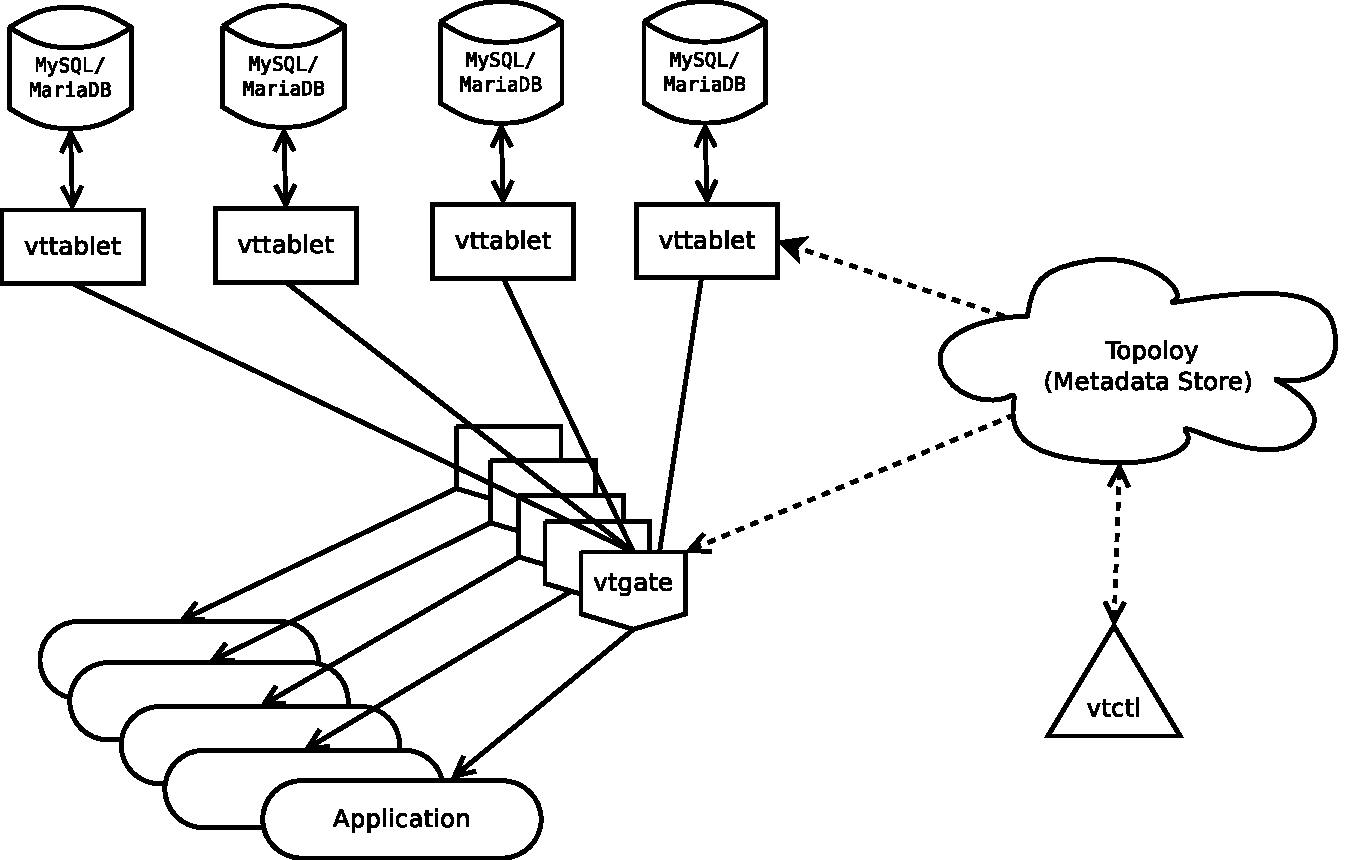
\includegraphics[scale=0.65]{VitessOverview.pdf}
\end{center}
\end{figure}


Vitess consists of a number servers, command line utilities, and a consistent
metadata store. Taken together, they allow you to serve more database traffic,
and add features like sharding, which normally you would have to implement in your
application.

\index{vttable}{\textbf{vttablet}} is a server that sits in front of a MySQL database, making it more
robust and available in the face of high traffic. Among other things, it adds a
connection pool, has a row based cache, and it rewrites SQL queries to be safer
and nicer to the underlying database.


\index{vtgate}{\textbf{vtgate}} is a very light proxy that routes database traffic from your app to the
right vttablet, basing on the sharding scheme, latency required, and health of
the vttablets. This allows the client to be very simple, as all it needs to be
concerned about is finding the closest vtgate.

The \index{topology}{\textbf{topology}} is a metadata store that contains information about running
servers, the sharding scheme, and replication graph. It is backed by a
consistent data store, like \href{http://zookeeper.apache.org/}{Apache ZooKeeper}.
The topology backends are plugin based, allowing you to write your own if
ZooKeeper doesn't fit your needs. You can explore the topology through
\index{vtctld}{\textbf{vtctld}}, a webserver (not shown in the diagram).

\index{vtctl}{\textbf{vtctl}} a command line utility that allows a human or a script to easily
interact with the system.

All components communicate using a lightweight RPC system based on
\href{http://bsonspec.org/}\index{BSON}{\textbf{BSON}}. The RPC system is plugin based, so you can easily
write your own backend (at Google we use a Protocol Buffers based protocol). We
provide a client implementation for three languages: Python, Go, and Java.
Writing a client for your language should not be difficult, as it's a matter of
implementing only a few API calls (please send us a pull request if you do!).

To learn more, please click on the documentation links below.
You can also watch a \href{https://www.youtube.com/watch?v=midJ6b1LkA0}{9 minute introduction}
to Vitess \href{https://github.com/sougou}{sougou} prepared for Google I/O 2014.
There's also a longer presentation from the Fosdem `14 go devroom
(\href{https://github.com/youtube/vitess/blob/master/doc/Vitess2014.pdf?raw=true}{slides},
\href{http://youtu.be/qATTTSg6zXk}{video}).

\section{Trying it out}\hypertarget{trying-it-out}{}\label{trying-it-out}

Vitess is not entirely ready for unsupervised use yet. Some functionality is
still under development, APIs may change, and parts of the code are
undocumented. However, if you feel adventurous, you're more than welcome to try
it. We know that there are some rough edges, so please don't hesitate to reach out
to us through \href{https://groups.google.com/forum/\#!forum/vitess}{our mailing list}
if you run into any issues. Warnings aside, please take a look at Getting Started(~\ref{Getting-Started})

guide.

\section{Documentation}\hypertarget{documentation}{}\label{documentation}

\subsection{Intro}\hypertarget{intro}{}\label{intro}

\begin{itemize}
\item Helicopter overview(~\ref{Helicopter-Overview}):  high level overview of Vitess that should tell you whether Vitess is for you.
\item FAQ(~\ref{Vitess-FAQ}):Vitess Frequently Asked Questions.
\item Vision(~\ref{Motivation-and-Vision}): principles guiding the design of Vitess.
\end{itemize}

\subsection{Using Vitess}\label{using-vitess}

\begin{itemize}
\item Getting Started(~\ref{Getting-Started}):  how to set your environment to work with Vitess.
\item Tools and Servers(~\ref{Tools-and-Servers}):  all Vitess tools and servers.
\item Vttablet(~\ref{Vttablet}):  information about the most important Vitess server.
\item Reparenting(~\ref{Reparenting}):  performing master failover.
\item Resharding(~\ref{Resharding}):  adding more shards to your cluster.
\item Preparing for production(~\ref{Production-Setup}): (wip).
\item Schema management(~\ref{Schema-Management}): managing your database schema using Vitess.
\end{itemize}

\subsection{Reference}

\begin{itemize}
\item General Concepts (~\ref{Concepts}):
\item Zookeeper data (~\ref{ZookeeperData}):
\item Serving graph (~\ref{Serving-Graph}):
\item Replication Graph (~\ref{Replication-Graph}):
\end{itemize}

\section{License}\hypertarget{license}{}\label{license}

Unless otherwise noted, the vitess source files are distributed
under the BSD-style license found in the LICENSE file.


%Intro
\chapter{Vitess Introduction}
\section{Helicopter overview}\label{Helicopter-Overview}

This is a very high level overview of Vitess. It doesn’t get into the technical
details – it’s goal is to help you understand if Vitess can solve your problems,
and what kind of effort it would require for you to start using Vitess.

\subsection{When do you need Vitess?}\hypertarget{when-do-you-need-vitess}{}\label{when-do-you-need-vitess}

\begin{itemize}
\item You store all your data in a MySQL database, and have a significant number of
  clients. At some point, you start getting Too many connections errors from
  MySQL, so you have to change the max\_connections system variable. Every MySQL
  connection has a memory overhead, which is just below 3 MB in the default
  configuration. If you want 1500 additional connections, you will need over 4 GB
  of additional RAM – and this is not going to be contributing to faster queries.
\item From time to time, your developers make mistakes. For example, they make your
  app issue a query without setting a LIMIT, which makes the database slow for
  all users. Or maybe they issue updates that break statement based replication.
  Whenever you see such a query, you react, but it usually takes some time and
  effort to get the story straight.
\item You store your data in a MySQL database, and your database has grown
  uncomfortably big. You are planning to do some horizontal sharding. MySQL
  doesn’t support sharding, so you will have write the code to perform the
  sharding, and then bake all the sharding logic into your app.
\item You run a MySQL cluster, and use replication for availability: you have a master
  database and a few replicas, and in the case of a master failure some replica
  should become the new master. You have to manage the lifecycle of the databases,
  and communicate the current state of the system to the application.
\item You run a MySQL cluster, and have custom database configurations for different
  workloads. There’s the master where all the writes go, fast read-only replicas
  for web clients, slower read-only replicas for batch jobs, and another kind of
  slower replicas for backups. If you have horizontal sharding, this setup is
  repeated for every shard. The code that your app uses to find the right
  database is rather complicated, and you have to deal with constantly updating
  the configuration.
\end{itemize}

If your MySQL installation is similar to any of the three scenarios described
above, you may benefit from taking a closer look at Vitess. YouTube suffered
from an extreme case of all of these problems – we serve a lot of traffic – and
Vitess helped us alleviate them.

\subsection{How Vitess can help?}\hypertarget{how-vitess-can-help}{}\label{how-vitess-can-help}

\subsubsection{Connection pooling}\hypertarget{connection-pooling}{}\label{connection-pooling}

Instead of using MySQL’s protocol, clients connect to Vitess uses its almost
stateless, BSON based protocol. These connections are very lightweight (around
32 KB per connections), which means our servers can handle thousands of them
without breaking a sweat. These connections are efficiently mapped to a pool of
MySQL connections thanks to Go’s awesome concurrency support.

\subsubsection{Handling queries}\hypertarget{handling-queries}{}\label{handling-queries}

When Vitess gets a query, it goes through a SQL parser, which informs the
decision how to proceed with the query. If the query looks like it could have an
avoidable negative impact on the performance, it will be rewritten according to
a configurable set of rules. For example, queries without a limit will get a
default limit of 10 thousand rows. If at the time a client issues a query the
exact same query is already in flight, the database will do the work only once,
returning the same result to both clients.

\subsubsection{Sharding}\hypertarget{sharding}{}\label{sharding}

Vitess has sharding built in, and it facilitates sharding with minimal downtime.
For example, it supports split replication, in which the replication stream can
be divided in such a way that a future shard master will get only statements
that could possibly affect rows in its new shard. This allows us to perform a
resharding with only a few minutes of read-only downtime for the shard.

What is more, if you already have your own, custom sharding scheme in place,
Vitess is fine with that: you can easily keep using it for its other features.

\subsubsection{Workflow management}\hypertarget{workflow-management}{}\label{workflow-management}

Vitess can help you manage the lifecycle of your database instances. It supports
various scenarios, like master failover, backups, etc. – and all of them are
handled automatically, minimizing any necessary downtime.

\subsubsection{Limiting complexity}\hypertarget{limiting-complexity}{}\label{limiting-complexity}

All the metadata about the Vitess cluster (sharding scheme, running instances,
their health, work profile, etc.) is stored in the Topology, which is backed by
a consistent data store, like ZooKeeper. This means that the app’s cluster view
is always up to date and consistent for different clients. What is more, your
app doesn’t need to know anything about all this. It connects to Vitess servers
through vtgate, a lightweight proxy which handles routing the queries to the
appropriate instances. This allows the Vitess client to be extremely simple –
it’s just an implementation of a few API calls.

\subsection{Starting easy: vtocc}\hypertarget{starting-easy-vtocc}{}\label{starting-easy-vtocc}

If you are only interested in connection pooling and handling queries, you are
in luck: it should be simple to start using those features without making
significant changes to your infrastructure. All you need is to run vtocc in
front of your MySQL database, and change your app to use the Vitess client
instead of your MySQL driver. This is how we launched Vitess into production at
YouTube

\subsection{Going all the way: vttablet}\hypertarget{going-all-the-way-vttablet}{}\label{going-all-the-way-vttablet}

Getting a fully functional Vitess installation is a quite involved affair, and
it requires some planning.

\subsubsection{Topology backend}\hypertarget{topology-backend}{}\label{topology-backend}

Vitess needs to store its metadata in some place. This data storage needs to
have different properties than a regular database. It doesn’t need to support a
lot of traffic or data, but the data should be consistent and be able to survive
failures in the machines that host it (so, we are interested in Consistency and
Partition Tolerance from the \href{http://en.wikipedia.org/wiki/CAP\_theorem}{CAP
theorem}). This means that the ideal candidates for this role implement
\href{http://en.wikipedia.org/wiki/Paxos\_(computer\_science)}{Paxos} or something
equivalent.

Out of the box, Vitess supports \href{http://zookeeper.apache.org/}{Apache ZooKeeper}, which is a well battle tested
distributed lock service. If you have a reason not to use ZooKeeper, it should
be relatively easy to write a Vitess plugin to use something like Etcd, Consul,
or Doozer. At Google, for example, we use Chubby through the plugin mechanism.

\subsubsection{Preparing the data}\hypertarget{preparing-the-data}{}\label{preparing-the-data}

Vitess has the notion of a keyspace – a logical database that may consist of
many shards. If you handle sharding yourself or don’t need it, this is just a
matter of choosing a name (your database name is a reasonable choice). If you
want Vitess to handle sharding, or think you may need that in the future,
there’s a bit more work that you should do.

First, you have to think about your sharding scheme. This is quite a big topic
by itself, but the general idea is that data that is used together should be
kept on the same shard. For example, if your app deals with users and objects
created by those users, the user id is a good candidate to build your sharding
schema around. The choices you make about your sharding scheme are crucial. One
of the limitations of Vitess (and any other sharding solution for MySQL) is that
transactions will not work across shard boundaries.

Once you know what you want to base your sharding key on, you have to add this
data to the database. You should create an additional column in all your sharded
tables that’s big enough to contain a 64 bit integer and populate it.

\subsubsection{vttablets}\hypertarget{vttablets}{}\label{vttablets}

Now that the data is ready for Vitess, you can start launching vttablets. There
should be exactly one vttablet for every MySQL database, and you can tag
different vttablets for different kind of jobs. After you start an instance that
connects to its database, you let the system know about it by using vtctl, a
command line tool.

\subsubsection{Clients}\hypertarget{clients}{}\label{clients}

Your app won’t connect to the tablets directly – it will always go through
\index{vtgate}{vtgate}. There are many ways to setup vtgate. You can have a pool of them, or you
can start one per process or group of processes (it doesn’t consume much
resources). All your app needs to do is to use the Vitess client and somehow let
it know how to connect to a running vtgate instance.


\section{Motivation and Vision}\label{Motivation-and-Vision}

MySQL is an easy relational database to get started with.
It's easy to setup and has a short learning curve.
However, as your system starts to scale, it begins to run out of steam.
This is mainly because it's non-trivial to shard a MySQL database after the fact.
Among other problems, the growing number of connections also becomes an
unbearable overhead.

On the other end of the spectrum, there are NoSQL databases.
However, they suffer from problems that mainly stem from the fact that they're new.
Those who have adopted them have struggled with the lack of secondary indexes,
table joins and transactions.

Vitess tries to bring the best of both worlds by trading off
some of MySQL's consistency features in order to achieve the
kind of scalability that NoSQL databases provide.

\subsubsection{Priorities}\hypertarget{priorities}{}\label{priorities}

\begin{itemize}
\item \emph{Scalability}: This is achieved by replication and sharding.
\item \emph{Efficiency}: This is achieved by a proxy server (vttablet) that mediates
all queries and connections.
It also utilizes a more efficient rowcache to short-cut some of the queries.
This effectively increases a typical MySQL's serving capacity.
\item \emph{Manageability}: As soon as you add replication and sharding that span
across multiple data centers, the number of servers spirals out of control.
Vitess provides a set of tools backed by a \index{lockserver}{\textbf{lockserver}} (zookeeper) to
track and administer them.
\item \emph{Simplicity}: As the complexity grows, it's important to hide this
from the application.
The vtgate servers give you a unified view of the fleet that makes
it feel like you're just interacting with one database.
\end{itemize}

\subsubsection{Trade-offs}\hypertarget{trade-offs}{}\label{trade-offs}

Scalability and availability require some trade-offs:
\begin{itemize}
\item  \emph{Consistency}: In a typical web application, not all reads have to be
fully consistent.

Vitess lets you specify the kind of consistency you want on your read.
It's generally recommended that you use replica reads as they're easier to scale.
You can always request for master reads if you want up-to-date data.
You can also additionally perform 'for update' reads that ensure that
a row will not change until you've committed your changes.
\item  \emph{Transactions}: Relational transactions are prohibitively expensive
across distributed systems.
Vitess eases this constraint and guarantees transactional integrity
'per keyspace id', which is restricted to one shard.
Heuristically, this tends to cover most of an application's transactions.
For the few cases that don't, you can sequence your changes in such a way
that the system looks consistent even if a distributed transaction fails
in the middle.
\item  \emph{Latency}: There is some negligible latency introduced by the proxy servers.
However, they make up for the fact that you can extract more throughput from
MySQL than you would otherwise be able to without them.
\end{itemize}

\subsubsection{Preserved MySQL features}\hypertarget{preserved-mysql-features}{}\label{preserved-mysql-features}

Since the underlying storage layer is still MySQL, we still get to preserve
its other important features:
\begin{itemize}
\item  \emph{Indexes}: You can create secondary indexes on your tables. This allows you
to efficiently query rows using more than one key.
\item  \emph{Joins}:  MySQL allows you to split one-to-many and many-to-many relational data
into separate tables, and lets you join them on demand.
\end{itemize}
This flexibility generally results in more efficient storage as each piece of
data is stored only once, and fetched only if needed.

\subsubsection{The Vitess spectrum}\hypertarget{the-vitess-spectrum}{}\label{the-vitess-spectrum}

The following diagram illustrates where vitess fits in the spectrum of storage solutions:

\begin{figure}[H]
\caption{Vitess Spectrum}
\label{fig:Vitess Spectrum}
\begin{center}
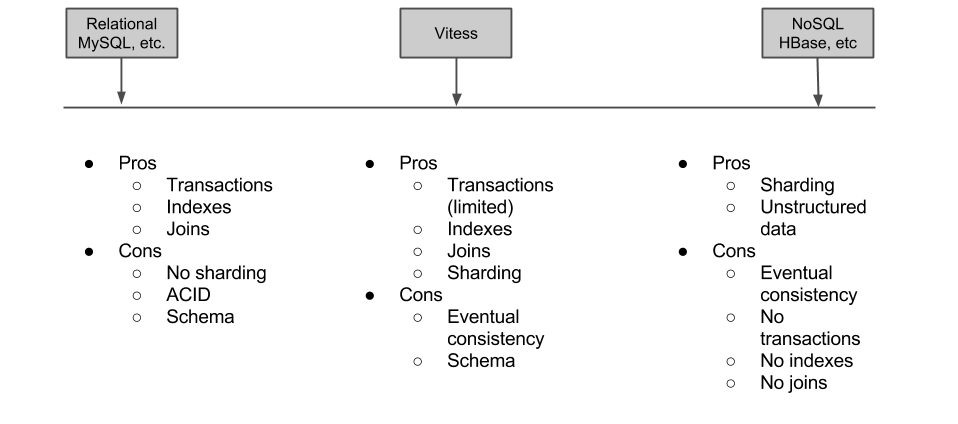
\includegraphics[scale=0.65]{VitessSpectrum.pdf}
\end{center}
\end{figure}





\section{Frequently Asked Questions}\label{Vitess-FAQ}

\subsection{Is Vitess used at Google?}\label{is-vitess-used-at-google}

Yes, Vitess has been used to serve all YouTube database traffic since
2011.

\subsection{Why not do it inside MySQL?}\label{why-not-do-it-inside-mysql}

MySQL is really good at what it does: serving queries with a low
latency, on a single server. However, it was not designed to do a lot
of the things at the scale that we need at YouTube. Including the
changes we needed inside MySQL itself would have been a huge
project. Additionally, it’s a large C++ codebase that’s almost 20
years old, which means that making changes is more complicated than we
would like. We decided to correct or enforce the behaviors we
needed from the outside.

\subsection{Why is it written in Go?}\hypertarget{why-is-it-written-in-go}{}\label{why-is-it-written-in-go}

Go is a language that hits the sweet spot in terms of expressiveness
and performance: it’s almost as expressive as Python, very
maintainable, but its performance is in the same range as Java (close
to C++ in certain cases). What is more, the language is extremely well
suited for concurrent programming, and it has a very high quality
standard library.

\subsection{Why not use X (where X is usually a NoSQL database) instead of putting effort into scaling MySQL?}\label{why-not-use-x-where-x-is-usually-a-nosql-database-instead-of-putting-effort-into-scaling-mysql}

Every database has its performance profile, meaning that some types of
queries usually run faster than other. Because of that, migrating from
one datastore to another involves a lot more work than just copying
the data and writing equivalent queries. If you need high performance,
you need to rethink how your app accesses its data. MySQL’s low
latency is very hard to match. Moreover, even if it has some quirks,
those quirks are usually pretty well understood.

\subsection{What’s up with the name, Vitess?}\label{whats-up-with-the-name-vitess}

Vitess was originally named \vconcepts{\emph{Voltron}}, but we decided to change it
before making it Open Source to avoid infringing any
trademarks. Still, we wanted a name that would allow us to keep using
the prefix VT in our code. \emph{Vitesse} means speed in French – and we
dropped the final E to make it easier to find using Google (also, it
looks much cooler without the E!).

\subsection{Why are you using ZooKeeper instead of Etcd/Doozer/Consul/etc?}\hypertarget{why-are-you-using-zookeeper-instead-of-etcddoozerconsuletc}{}\label{why-are-you-using-zookeeper-instead-of-etcddoozerconsuletc}

The topology is a crucial part of our infrastructure, so we didn’t
want to take any risks with it. ZooKeeper may have some rough edges
and not be very easy to set up, but it’s battle tested, so we know we
can rely on it. Of course, you are free to write a plugin to use your
lock service of choice – we would appreciate if you contributed the
code back.

\subsection{Is the Vitess used at Google the same as the Open Source version?}\hypertarget{is-the-vitess-used-at-google-the-same-as-the-open-source-version}{}\label{is-the-vitess-used-at-google-the-same-as-the-open-source-version}

Mostly. The core functionality remains unchanged, but we add some code
to take advantage of Google’s infrastructure (so we can use \cite{web:chubby} Chubby,
the Protocol Buffers based RPC system, etc.). Our philosophy is “Open
Source first” – when we develop a new feature, we first make it work
in the Open Source tree, and only then write a plugin that makes use
of Google specific technologies. We believe this is very important to
keep us honest, and to ensure that the Open Source version of Vitess
is as high quality as the internal one. The vast majority of our
development takes place in the open, on GitHub. This also means that
Vitess is built with extensibility in mind – it should be pretty
straightforward to adjust it to the needs of your infrastructure.


\section{Contributing to Vitess}\hypertarget{contributing-to-vitess}{}\label{contributing-to-vitess}

If you'd like to make simple contributions to Vitess, we recommend that you fork
the repository and submit pull requests. If you'd like to make larger or ongoing
changes, you'll need to follow a similar set of processes and rules that the
Vitess team follows.

\subsubsection{Prerequisites}\hypertarget{prerequisites}{}\label{prerequisites}

\begin{itemize}
\item \href{https://github.com/youtube/vitess/blob/master/doc/GettingStarted.markdown}{Install vitess}
\item The vitess team uses appspot for code reviews. You'll need to create an account at http://codereview.appspot.com.
\item Fork the vitess repository, say https://github.com/myfork/vitess.
\item Download \href{https://code.google.com/p/rietveld/wiki/UploadPyUsage}{upload.py} and put it in your path.
\end{itemize}

\subsection{Small changes}\hypertarget{small-changes}{}\label{small-changes}

For small, well contained changes, just send us a
\href{https://help.github.com/articles/using-pull-requests}{pull request}.

\subsection{Bigger changes}\hypertarget{bigger-changes}{}\label{bigger-changes}

If you are planning to make bigger changes or add serious features to Vitess, we
ask you to follow our code review process.

\subsubsection{Recommended Git flow: single contributor}\hypertarget{recommended-git-flow-single-contributor}{}\label{recommended-git-flow-single-contributor}

Use your fork as a push-only staging ground for submitting pull requests. The
assumption is that you'll never have to fetch from the fork. If this is the
case, all you have to do is configure your local repository to pull from
youtube, and push to myfork. This can be achieved as follows:

{\tt 
\ensuremath{\sim}/...vitess\textgreater{} git remote -v
origin  git@github.com:youtube/vitess.git (fetch)
origin  git@github.com:youtube/vitess (push)
\ensuremath{\sim}/...vitess\textgreater{} git remote set-url --push origin git@github.com:myfork/vitess
\ensuremath{\sim}/...vitess\textgreater{} git remote -v
origin  git@github.com:youtube/vitess.git (fetch)
origin  git@github.com:myfork/vitess (push)
}

The limitation of this configuration is that you can only pull from the youtube
repository. The {\tt git pull} command will {\tt fetch} from youtube/vitess and {\tt merge}
into your master branch.

On the other hand, {\tt git push} will push into your myfork/vitess remote.

The advantage of this workflow is that you don't have to worry about specifying
where you're pulling from or pushing to because the default settings \emph{do the
right thing}.

\subsubsection{Recommended Git flow: multiple contributors}\hypertarget{recommended-git-flow-multiple-contributors}{}\label{recommended-git-flow-multiple-contributors}

If more than one of you plan on contributing through a single fork, then you'll
need to follow a more elaborate scheme of setting up multiple remotes and
manually managing merges:

{\tt 
\ensuremath{\sim}/...vitess\textgreater{} git remote -v
origin  git@github.com:youtube/vitess.git (fetch)
origin  git@github.com:youtube/vitess.git (push)
\ensuremath{\sim}/...vitess\textgreater{} git remote add myfork git@github.com:myfork/vitess.git
\ensuremath{\sim}/...vitess\textgreater{} git remote -v
myfork  git@github.com:myfork/vitess.git (fetch)
myfork  git@github.com:myfork/vitess.git (push)
origin  git@github.com:youtube/vitess.git (fetch)
origin  git@github.com:youtube/vitess.git (push)
}

With this setup, commands like {\tt git pull} and {\tt git push} with default settings
are not recommended. You will be better off using {\tt git fetch} and {\tt git merge},
which let you micromanage your remote interactions. For example, you'll need to
{\tt git push myfork} to explicitly push your changes to myfork.

\subsubsection{Changes and code reviews}\hypertarget{changes-and-code-reviews}{}\label{changes-and-code-reviews}

We recommend that you make your changes in a separate branch.
Make sure you're on the master branch when you create it.

{\tt 
\ensuremath{\sim}/...vitess\textgreater{} git status
\# On branch master
\# Your branch is up-to-date with 'origin/master'.
\#
nothing to commit, working directory clean
\ensuremath{\sim}/...vitess\textgreater{} git checkout -b newfeature
Switched to a new branch 'newfeature'
}
Once your changes are ready for review and committed into your branch,
you can run the createcl tool, for example:
{\tt 
createcl -r alainjobart
}
This command will automatically run a diff of the current branch {\tt newfeature}
against {\tt master} and create an appspot code review with {\tt alainjobart} as
reviewer. vitess-issues will be cc'd. If necessary, createcl allows you to
specify the exact versions to diff. (but we recommend that you don't use those).

After getting feedback about your code, you can update the code by calling

{\tt 
createcl -i 12345
}

with the actual id of your change instead of 12345.

During your feature development, you can fetch and merge new changes from the main youtube repository.
If you choose to do so, make sure you merge the changes to both the {\tt master} and {\tt newfeature} branches.
In the sole contributor case, your commands will look like this:
{\tt 
git checkout master
git pull
git checkout newfeature
git merge master
}
Once your change is approved, push and submit it as a pull request:
{\tt 
git checkout master
git merge newfeature
git push
}
The above commands will merge {\tt newfeature} into {\tt master} and push the changes to the myfork remote.
You can then go to https://github.com/myfork/vitess to submit the branch as your pull request.
If done correctly, only your changes will show up in the pull request.
github will cancel out changes you merged from youtube master, unless you resolved merge conflicts.

If necessary, you can work on multiple branches at the same time.
When the time comes to submit, you just have to merge the branch onto {\tt master} and push.

\subsection{Other Git setups}\hypertarget{other-git-setups}{}\label{other-git-setups}

As you can see above, the only requirement from the Vitess team is that you send
your code reviews through appspot, and then submit the same changes as a pull
request.

Our workflow recommendation is mainly to simplify your life. If you prefer to
use a different workflow, you can choose to do so as long as you can figure out
a way to meet the necessary requirements.


% Using Vitess
\chapter{Using Vitess}
 \section{Getting Started}\hypertarget{getting-started}{}\label{getting-started}

If you run into issues or have questions, you can use our mailing list: vitess@googlegroups.com.

\subsection{Dependencies}\hypertarget{dependencies}{}\label{dependencies}

\begin{itemize}
\item We currently develop on Ubuntu 12.04 and 14.04.
\item You'll need some kind of Java Runtime (for ZooKeeper).
We use OpenJDK (\emph{sudo apt-get install openjdk-7-jre}).
\item \href{http://golang.org}{Go} 1.2+: Needed for building Vitess.
\item \href{https://mariadb.org/}{MariaDB}: We currently develop with version 10.0.13.
Other 10.0.x versions may also work.
\item \href{http://zookeeper.apache.org/}{ZooKeeper}: By default, Vitess
uses Zookeeper as the lock service. It is possible to plug in
something else as long as the new service supports the
necessary API functions.
\item \href{http://memcached.org}{Memcached}: Used for the rowcache.
\item \href{http://python.org}{Python}: For the client and testing.
\end{itemize}

\subsection{Building}\hypertarget{building}{}\label{building}

\href{http://golang.org/doc/install}{Install Go}.

\href{https://downloads.mariadb.org/}{Install MariaDB}.
You can use any installation method (src/bin/rpm/deb),
but be sure to include the client development headers (\textbf{libmariadbclient-dev}).

Then download and build Vitess. Note that the value of MYSQL\_FLAVOR is case-sensitive.
If the mysql\_config command from libmariadbclient-dev is not on the PATH,
you'll need to \emph{export VT\_MYSQL\_ROOT=/path/to/mariadb} before running bootstrap.sh,
where mysql\_config is found at /path/to/mariadb/\textbf{bin}/mysql\_config.

{\tt sh
cd \$WORKSPACE
sudo apt-get install make automake libtool memcached python-dev python-mysqldb libssl-dev g++ mercurial git pkg-config bison curl
git clone https://github.com/youtube/vitess.git src/github.com/youtube/vitess
cd src/github.com/youtube/vitess
export MYSQL\_FLAVOR=MariaDB
./bootstrap.sh
. ./dev.env
make build
}

\subsection{Testing}\hypertarget{testing}{}\label{testing}

The full set of tests included in the default \emph{make} and \emph{make test} targets
is intended for use by Vitess developers to verify code changes.
These tests simulate a small cluster by launching many servers on the local
machine, so they require a lot of resources (minimum 8GB RAM and SSD recommended).

If you are only interested in checking that Vitess is working in your
environment, you can run a set of lighter tests:

{\tt sh
make site\_test
}

\subsubsection{Common Test Issues}\hypertarget{common-test-issues}{}\label{common-test-issues}

Many common failures come from running the full developer test suite
(\emph{make} or \emph{make test}) on an underpowered machine. If you still get
these errors with the lighter set of site tests (\emph{make site\_test}),
please let us know on the mailing list.

\paragraph{Node already exists, port in use, etc.}\hypertarget{node-already-exists-port-in-use-etc}{}\label{node-already-exists-port-in-use-etc}

Sometimes a failed test may leave behind orphaned processes.
If you use the default settings, you can find these by looking for
\emph{vtdataroot} in the command line, since every process is told to put
its files there with a command line flag. For example:

{\tt sh
pgrep -f -l '(vtdataroot\textbar{}VTDATAROOT)' \# list Vitess processes
pkill -f '(vtdataroot\textbar{}VTDATAROOT)' \# kill Vitess processes
}

\paragraph{Too many connections to MySQL, or other timeouts}\hypertarget{too-many-connections-to-mysql-or-other-timeouts}{}\label{too-many-connections-to-mysql-or-other-timeouts}

This often means your disk is too slow. If you don't have access to an SSD,
you can try \href{TestingOnARamDisk.markdown}{testing against a ramdisk}.

\paragraph{Connection refused to tablet, MySQL socket not found, etc.}\hypertarget{connection-refused-to-tablet-mysql-socket-not-found-etc}{}\label{connection-refused-to-tablet-mysql-socket-not-found-etc}

This could mean you ran out of RAM and a server crashed when it tried to allocate more.
Some of the heavier tests currently require up to 8GB RAM.

\paragraph{Connection refused in zkctl test}\hypertarget{connection-refused-in-zkctl-test}{}\label{connection-refused-in-zkctl-test}

This could indicate that no Java Runtime is installed.

\paragraph{Running out of disk space}\hypertarget{running-out-of-disk-space}{}\label{running-out-of-disk-space}

Some of the larger tests use up to 4GB of temporary space on disk.

\subsection{Setting up a cluster}\hypertarget{setting-up-a-cluster}{}\label{setting-up-a-cluster}

\subsection{TODO}\hypertarget{TODO}{}\label{TODO}
TODO: Expand on all sections
\begin{itemize}
\item  Setup zookeeper
\item  Start a MySql instance
\item  Start vttablet
\item  Start vtgate
\item  Write a client
\item  Test
\end{itemize}


 \section{Tools and servers}\hypertarget{tools-and-servers}{}\label{tools-and-servers}

The vitess tools and servers are designed to help you even
if you start small, and scale all the way to a complete fleet
of databases.

In the early stages, connection pooling, rowcache and other
efficiency features of vttablet help you get more from your
existing hardware.
As things scale out, the automation tools start to become handy.

\subsubsection{vtctl}\hypertarget{vtctl}{}\label{vtctl}

vtctl is the main tool for performing administrative operations.
It can be used to track shards, replication graphs and
db categories.
It's also used to initiate failovers, reshard, etc.

As vtctl performs operations, it updates the necessary
changes to the lockserver (zookeeper).
The rest of the vitess servers observe those changes
and react accordingly.
For example, if a master database if failed over to a new
one, the vitess servers will see the change and redirect
future writes to the new master.

\subsubsection{vttablet}\hypertarget{vttablet}{}\label{vttablet}

One of vttablet's main function is to be a proxy to MySQL.
It performs tasks that attempt to maximize throughput as
well as to protect MySQL from harmful queries. There is
one vttablet per MySQL instance.

vttablet is also capable of executing necessary management
tasks initiated from vtctl.
It also provides streaming services that are used for
filtered replication and data export.

\subsubsection{vtocc}\hypertarget{vtocc}{}\label{vtocc}

Vtocc is the previous version of vttablet. It handles query management
(same as vttablet) but is not part of a larger system, it's a standalone
program that doesn't require a Topology Server. It is useful for
unit tests and when the only required feature is the query service
(with connection pooling, query de-dup, ...).

Note we may eventually produce a version of vttablet that runs
without a Topology Server, and use it instead of vtocc.

\subsubsection{vtgate}\hypertarget{vtgate}{}\label{vtgate}

vtgate's goal is to provide a unified view of the entire fleet.
It will be the server that applications will connect to for
queries. It will analyze, rewrite and route queries to various
vttablets, and return the consolidated results back to the client.

\subsubsection{vtctld}\hypertarget{vtctld}{}\label{vtctld}

vtctld is an HTTP server that lets you browse the information stored
in the lockserver.
This is useful for trouble-shooting, or to get a good high
level picture of all the servers and their current state.

\subsubsection{vtworker}\hypertarget{vtworker}{}\label{vtworker}

vtworker is meant to host long-running processes. It supports a plugin infrastructure, and offers libraries to easily pick tablets to use. We have developped:
- resharding differ jobs: meant to check data integrity during shard splits and joins.
- vertical split differ jobs: meant to check data integrity during vertical splits and joins.

It is very easy to add other checker processes for in-tablet integrity checks (verifying foreign key-like relationships), and cross shard data integrity (for instance, if a keyspace contains an index table referencing data in another keyspace).

\subsubsection{vtprimecache}\hypertarget{vtprimecache}{}\label{vtprimecache}

vtprimecache is a mysql cache primer for faster replication. If the single MySQL replication thread is falling behind, vtprimecache activates and starts reading the available relay logs. It then uses a few threads / connections to MySQL to execute modified statements and prime the MySQL buffer cache. The idea is for instance if an 'update table X where id=2' statement is going to be executed by the replication SQL thread 2 or 3 seconds from now, might as well execute a concurrent 'select from table X where id=2' now and prime the MySQL buffer cache. In practice, this shows a speed improvement in replication speed by 30 to 40 percents.

\subsubsection{Other support tools}\hypertarget{other-support-tools}{}\label{other-support-tools}

\begin{itemize}
\item \emph{mysqlctl}: manage MySQL instances.
\item \emph{zkctl}: manage ZooKeeper instances.
\item \emph{zk}: command line ZooKeeper client and explorer.
\end{itemize}

\subsection{Vitess components block diagram}\hypertarget{vitess-components-block-diagram}{}\label{vitess-components-block-diagram}

\begin{figure}[H]
\caption{components block diagram}
\label{fig:Vitess Spectrum}
\begin{center}
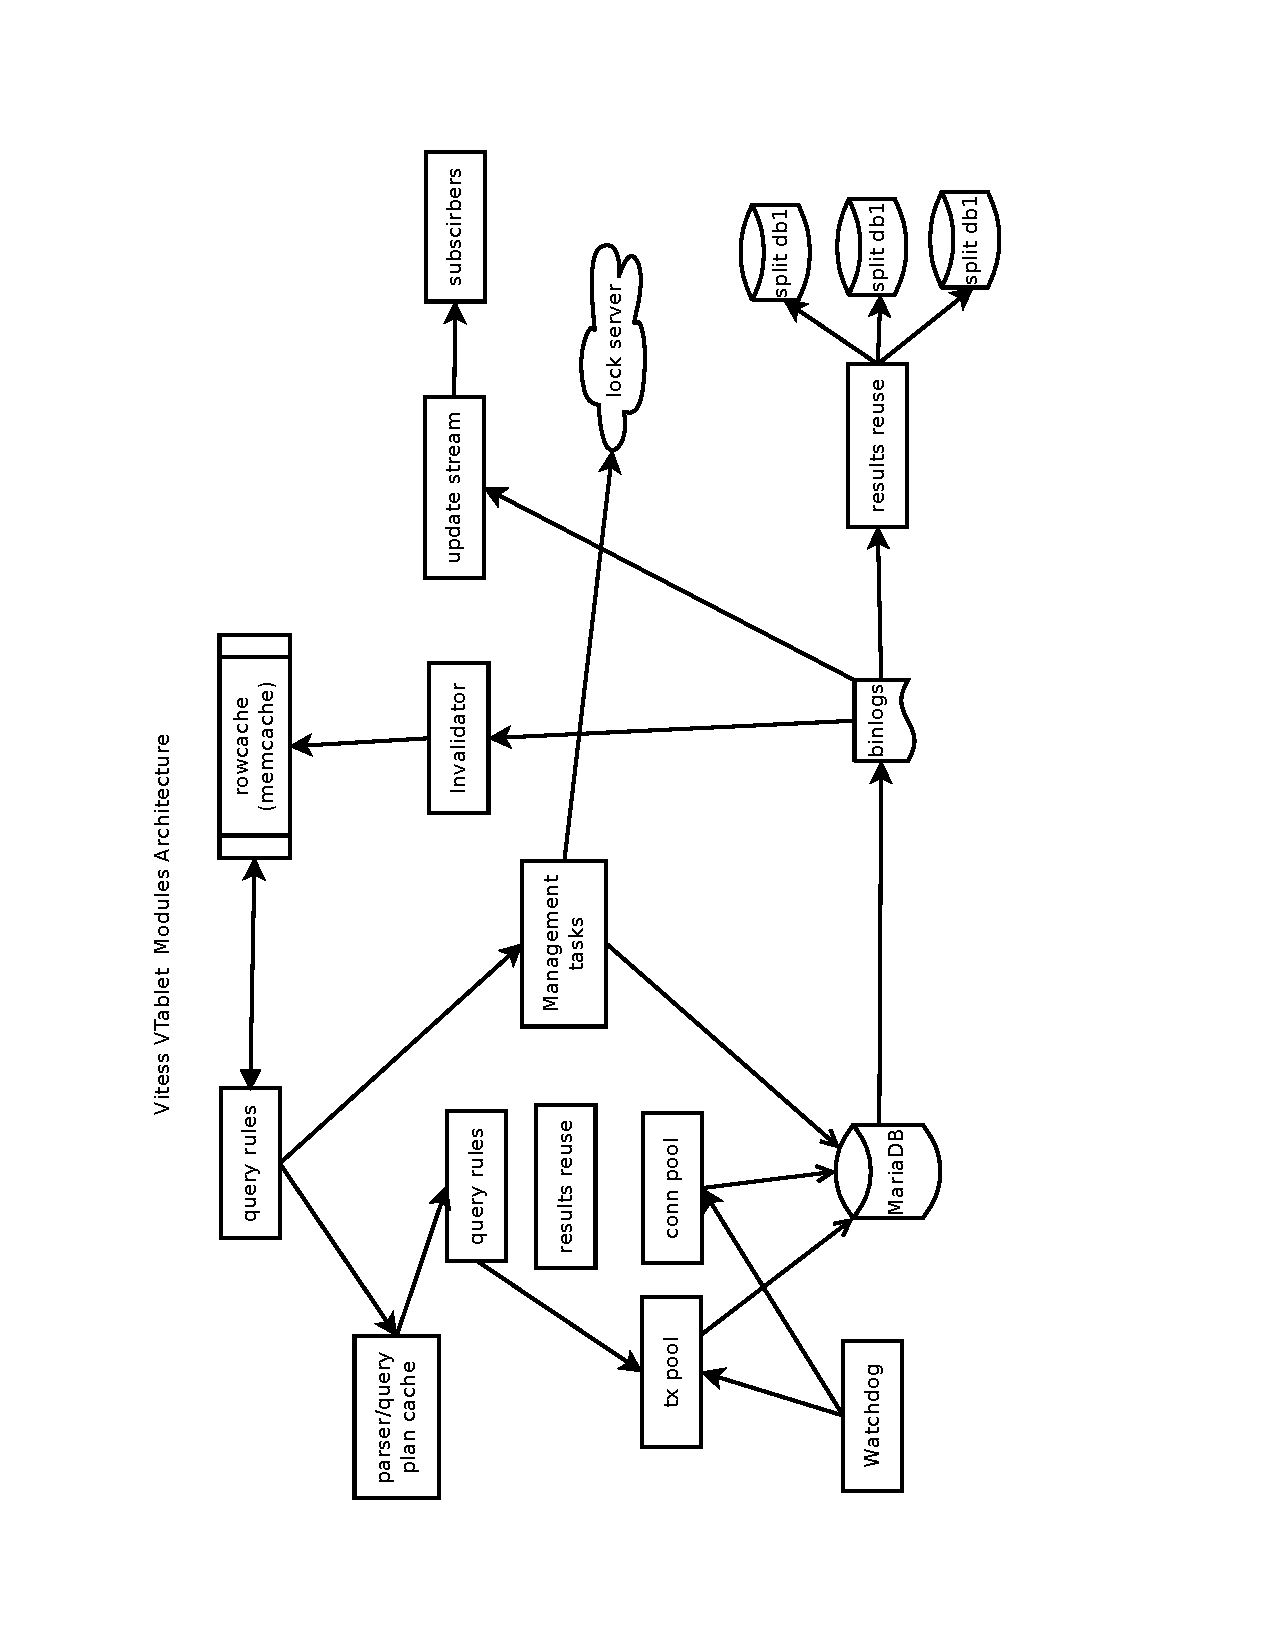
\includegraphics[scale=0.65]{VTTabletModules.pdf}
\end{center}
\end{figure}






 \section{vttablet}\hypertarget{vttablet}{}\label{vttablet}

Smart middleware sitting in front of MySQL and serving clients
requests.

\begin{itemize}
\item Connection pooling.
\item SQL parser: Although very close, the vtocc SQL parser is not SQL-92
compliant. It has left out constructs that are deemed uncommon or
OLTP-unfriendly. It should, however, allow most queries used by a
well-behaved web application.
\item Query rewrite and sanitation (adding limits, avoiding non-deterministic updates).
\item Query consolidation: reuse the results of an in-flight query to any
subsequent requests that were received while the query was still
executing.
\item Rowcache: the mysql buffer cache is optimized for range scans over
indices and tables. Unfortunately, it’s not good for random access
by primary key. The rowcache will instead maintain a row based cache
(using \href{http://memcached.org/}{memcached} as its backend) and keep it
consistent by fielding all DMLs that could potentially affect them.
\item Update stream: A server that streams the list of rows that are changing
in the database, which can be used as a mechanism to continuously export
the data to another data store.
\item Integrated query killer for queries that take too long to return
data.
\item Discard idle backend connections to avoid offline db errors.
\item Transaction management: Ability to limit the number of concurrent
transactions and manage deadlines.
\end{itemize}

 \section{Reparenting}\label{Reparenting}

This document describes the reparenting features of Vitess. Reparenting is used when the master for a Shard is
changing from one host to another. It can be triggered (for maintenance for instance) or happen automatically
(based on the current master dying for instance).

Two main types of reparenting supported by Vitess are Active Reparents (the Vitess toolchain is handing it all)
and External Reparents (another tool is responsible for reparenting, and the Vitess toolchain just update its
internal state.

\subsection{Active Reparents}\label{active-reparents}

They are triggered by using the 'vtctl ReparentShard' command. See the help for that command. It currently doesn't use transaction GroupId.

\subsection{External Reparents}\label{external-reparents}

In this part, we assume another tool has been reparenting our servers. We then trigger the
'vtctl ShardExternallyReparented' command.

The flow for that command is as follows:
\begin{itemize}
\item  the shard is locked in the global topology server.
\item  we read the Shard object from the global topology server.
\item  we read all the tablets in the replication graph for the shard. We also check the new master is in the map. Note we allow partial reads here, so if a data center is down, as long as the data center containing the new master is up, we keep going.
\item  we call the 'SlaveWasPromoted' remote action on the new master. This remote action makes sure the new master is not a MySQL slave of another server (the 'show slave status' command should not return anything, meaning 'reset slave' should ave been called).
\item  for every host in the replication graph, we call the 'SlaveWasRestarted' action. It takes as paremeter the address of the new master. On each slave, it executes a 'show slave status'. If the master matches the new master, we update the topology server record for that tablet with the new master, and the replication graph for that tablet as well. If it doesn't match, we keep the old record in the replication graph (pointing at whatever master was there before). We optionally Scrap tablets that bad (disabled by default).
\item  if a smaller percentage than a configurable value of the slaves works (80\% be default), we stop here.
\item  we then update the Shard object with the new master.
\item  we rebuild the serving graph for that shard. This will update the 'master' record for sure, and also keep all the tablets that have successfully reparented.
\end{itemize}

Optional Flags:
\begin{itemize}
\item  -accept-success-percents=80: will declare success if more than that many slaves can be reparented
\item  -continue\_on\_unexpected\_master=false: if a slave has the wrong master, we'll just log the error and keep going
\item  -scrap-stragglers=false: will scrap bad hosts
\end{itemize}

Failure cases:

\begin{itemize}
\item The global topology server has to be available for locking and modification during this operation. If not, the operation will just fail.
\item If a single topology server is down in one data center 9and it's nto the master data center), the tablets in that data center will be ignored by the reparent. Provided it doesn't trigger the 80\% threshold, this is not a big deal. When the topology server comes back up, just re-run 'vtctl InitTablet' on the tablets, and that will fix their master record.
\item If scrap-straggler is false (the default), a tablet that has the wrong master will be kept in the replication graph with its original master. When we rebuild the serving graph, that tablet won't be added, as it doesn't have the right master.
\item if more than 20\% of the tablets fails, we don't update the Shard object, and don't rebuild. We assume something is seriously wrong, and it might be our process, not the servers. Figuring out the cause and re-running 'vtctl ShardExternallyReparented' should work.
\item if for some reasons none of the slaves report the right master (replication is going through a proxy for instance, and the master address is not what the clients are showing in 'show slave status'), the result is pretty bad. All slaves are kept in the replication graph, but with their old (incorrect) master. Next time a Shard rebuild happens, all the servers will disappear. At that point, fixing the issue and then re-parenting will work.
\end{itemize}

\subsection{Reparenting And Serving Graph}\label{reparenting-and-serving-graph}

When reparenting, we shuffle servers around. A server may get demoted, another promoted, and some servers may end up with the wrong master in the replication graph, or scrapped.

It is important to understand that when we build the serving graph, we go through all the servers in the replication graph, and check their masters. If their master is the one we expect (because it is in the Shard record), we keep going and add them to the serving graph. If not, they are skipped, and a warning is displayed.

When such a slave with the wrong master is present, re-running 'vtclt InitTablet' with the right parameters will fix the server. So the order of operations should be to fix mysql replication, make sure it is caught up, run 'vtctl InitTablet', and maybe restart vttablet if needed.

Alternatively, if another reparent happens, and the bad slave recovers and now replicates from the new master, it will be re-added, and resume proper operation.

The old master for reparenting is a specific case. If it doesn't have the right master during the reparent, it will be scrapped (because it's not in the replication graph at all, so it would get lost anyway).


 \section{Resharding}\hypertarget{resharding}{}\label{resharding}

In Vitess, resharding describes the process of re-organizing data dynamically, with very minimal downtime (we manage to
completely perform most data transitions with less than 5 seconds of read-only downtime - new data cannot be written,
existing data can still be read).

\subsection{Process}\hypertarget{process}{}\label{process}

The process to achieve this goal is composed of the following steps:

\begin{itemize}
\item pick the original shard(s)
\item pick the destination shard(s) coverage
\item create the destination shard(s) tablets (in a mode where they are not used to serve traffic yet)
\item bring up the destination shard(s) tablets, with read-only masters.
\item backup and split the data from the original shard(s)
\item merge and import the data on the destination shard(s)
\item start and run filtered replication from original to destination shard(s), catch up
\item move the read-only traffic to the destination shard(s), stop serving read-only traffic from original shard(s). This transition can take a few hours. We might want to move rdonly separately from replica traffic.
\item in quick succession:
   \begin{itemize}
   \item make original master(s) read-only
   \item flush filtered replication on all filtered replication source servers (after making sure they were caught up with their masters)
   \item wait until replication is caught up on all destination shard(s) masters
   \item move the write traffic to the destination shard(s)
   \item make destination master(s) read-write
   \end{itemize}
\item scrap the original shard(s)
\end{itemize}


\subsection{Applications}\hypertarget{applications}{}\label{applications}

The main application we currently support:


\begin{itemize}
\item in a sharded keyspace, split or merge shards (horizontal sharding)
\item in a non-sharded keyspace, break out some tables into a different keyspace (vertical sharding)
\end{itemize}

With these supported features, it is very easy to start with a single keyspace containing all the data (multiple tables),
and then as the data grows, move tables to different keyspaces, start sharding some keyspaces, ... without any real
downtime for the application.

\subsection{Scaling Up and Down}\hypertarget{scaling-up-and-down}{}\label{scaling-up-and-down}

Here is a quick table of what to do with Vitess when a change is required:

\begin{itemize}
\item uniformly increase read capacity: add replicas, or split shards
\item uniformly increase write capacity: split shards
\item reclaim free space: merge shards / keyspaces
\item increase geo-diversity: add new cells and new replicas
\item cool a hot tablet: if read access, add replicas or split shards, if write access, split shards.
\end{itemize}

\subsection{Filtered Replication}\hypertarget{filtered-replication}{}\label{filtered-replication}

The cornerstone of Resharding is being able to replicate the right data. Mysql doesn't support any filtering, so the
Vitess project implements it entirely:
\begin{itemize}
\item the tablet server tags transactions with comments that describe what the scope of the statements are (which keyspace\_id,
\item which table, ...). That way the MySQL binlogs contain all filtering data.
\item a server process can filter and stream the MySQL binlogs (using the comments).
\item a client process can apply the filtered logs locally (they are just regular SQL statements at this point).
\end{itemize}

 \section{Production setup}\label{Production-Setup}

Setting up vitess in production will depend on many factors.
Here are some initial considerations:
\begin{itemize}
\item \emph{Global Transaction IDs}: Vitess requires a version of MySQL that supports GTIDs, such as Google MySQL 5.1+, MariaDB 10.0+, or MySQL 5.6+. We currently support Google MySQL and MariaDB, with plans to add MySQL 5.6.
\item \emph{Firewalls}: Vitess tools and servers assume that they can open direct TCP connection to each other. If you have firewalls between your servers, you may have to add exceptions to allow these communications.
\item \emph{Authentication}: If you need authentication, you need to setup SASL, which is supported by Vitess.
\item \emph{Encryption:} Vitess RPC servers support SSL. TODO: Document how to setup SSL.
\item \emph{MySQL permissions}: Vitess currently assumes that all
application clients have uniform permissions.
The connection pooler opens a number of connections under
the same user (vt\_app), and rotates them for all requests.
Vitess management tasks use a different user name (vt\_dba),
which is assumed to have all administrative privileges.
\item \emph{Client Language}: We currently support
      Python and Go.
It's not too hard to add support for more languages,
and we are open to contributions in this area.
\end{itemize}

\subsection{Setting up Zookeeper}\hypertarget{setting-up-zookeeper}{}\label{setting-up-zookeeper}
\begin{enumerate}
\item Global zk setup:
TODO: Explain
\item Local zk setup:
TODO: Explain
\end{enumerate}
\subsection{Launch vttablets}\hypertarget{launch-vttablets}{}\label{launch-vttablets}

vttablet is designed to run on the same machine as mysql.
You'll need to launch one instance of vttablet for every MySQL instance you want to track.

TODO: Specify order and command-line arguments

\subsection{Launch vtgate(s)}\hypertarget{launch-vtgates}{}\label{launch-vtgates}

TODO: Explain


 \section{Schema Management}\label{Schema-Management}

The schema is the list of tables and how to create them. It is managed by vtctl.

\subsection{Looking at the Schema}\hypertarget{looking-at-the-schema}{}\label{looking-at-the-schema}

The following vtctl commands exist to look at the schema, and validate it's the same on all databases.



\begin{itemize}
\item GetSchema \textless{}zk tablet path\textgreater{} displays the full schema for a tablet
\item ValidateSchemaShard \textless{}zk shard path\textgreater{}
\item validate the master schema matches all the slaves.
\item ValidateSchemaKeyspace \textless{}zk keyspace path\textgreater{}
\end{itemize}
validate the master schema from shard 0 matches all the other tablets in the keyspace.

Example:

\begin{codesample2}
$ vtctl -wait-time=30s ValidateSchemaKeyspace /zk/global/vt/keyspaces/user
\end{codesample2}


\subsection{Changing the Schema}\hypertarget{changing-the-schema}{}\label{changing-the-schema}

Goals:
\begin{enumerate}
\item simplify schema updates on the fleet
\item minimize human actions / errors
\item guarantee no or very little downtime for most schema updates
\item do not store any permanent schema data in Topology Server, just use it for actions.
\item only look at tables for now (not stored procedures or grants for instance, although they both could be added fairly easily in the same manner)
\end{enumerate}

We’re trying to get reasonable confidence that a schema update is going to work before applying it. Since we cannot really apply a change to live tables without potentially causing trouble, we have implemented a Preflight operation: it copies the current schema into a temporary database, applies the change there to validate it, and gathers the resulting schema. After this Preflight, we have a good idea of what to expect, and we can apply the change to any database and make sure it worked.

The Preflight operation takes a sql string, and returns a SchemaChangeResult:
\begin{codesample4}
     type SchemaChangeResult struct \{
         Error        string
         BeforeSchema *SchemaDefinition
         AfterSchema  *SchemaDefinition
     \}
\end{codesample4}

The ApplySchema action applies a schema change. It is described by the following structure (also returns a SchemaChangeResult):
\begin{codesample4}
    type SchemaChange struct \{
     Sql              string
     Force            bool
     AllowReplication bool
     BeforeSchema     *SchemaDefinition
     AfterSchema      *SchemaDefinition
    \}
\end{codesample4}

And the associated ApplySchema remote action for a tablet. Then the performed steps are:
\begin{enumerate}
\item The database to use is either derived from the tablet dbName if UseVt is false, or is the \_vt database. A ‘use dbname’ is prepended to the Sql.
\item (if BeforeSchema is not nil) read the schema, make sure it is equal to BeforeSchema. If not equal: if Force is not set, we will abort, if Force is set, we’ll issue a warning and keep going.
\item if AllowReplication is false, we’ll disable replication (adding SET sql\_log\_bin=0 before the Sql).
\item We will then apply the Sql command.
\item (if AfterSchema is not nil) read the schema again, make sure it is equal to AfterSchema. If not equal: if Force is not set, we will issue an error, if Force is set, we’ll issue a warning.
\end{enumerate}

We will return the following information:
\begin{enumerate}
\item whether it worked or not (doh!)
\item BeforeSchema
\item  AfterSchema
\end{enumerate}

\subsubsection{Use case 1: Single tablet update:}\hypertarget{use-case-1-single-tablet-update}{}\label{use-case-1-single-tablet-update}

\begin{itemize}
\item we first do a Preflight (to know what BeforeSchema and AfterSchema will be). This can be disabled, but is not recommended.
\item we then do the schema upgrade. We will check BeforeSchema before the upgrade, and AfterSchema after the upgrade.
\end{itemize}

\subsubsection{Use case 2: Single Shard update:}\hypertarget{use-case-2-single-shard-update}{}\label{use-case-2-single-shard-update}

\begin{itemize}
\item need to figure out (or be told) if it’s a simple or complex schema update (does it require the shell game?). For now we'll use a command line flag.
\item in any case, do a Preflight on the master, to get the BeforeSchema and AfterSchema values.
\item in any case, gather the schema on all databases, to see which ones have been upgraded already or not. This guarantees we can interrupt and restart a schema change. Also, this makes sure no action is currently running on the databases we're about to change.
\item if simple:
\item nobody has it: apply to master, very similar to a single tablet update.
\item some tablets have it but not others: error out
\item if complex: do the shell game while disabling replication. Skip the tablets that already have it. Have an option to re-parent a the end.
\item Note the Backup, and Lag servers won't apply a complex schema change. Only the servers actively in the replication graph will.
\item the process can be interrupted at any time, restarting it as a complex schema upgrade should just work.
\end{itemize}

\subsubsection{Use case 3: Keyspace update:}\hypertarget{use-case-3-keyspace-update}{}\label{use-case-3-keyspace-update}

\begin{itemize}
\item Similar to Single Shard, but the BeforeSchema and AfterSchema values are taken from the first shard, and used in all shards after that.
\item We don't know the new masters to use on each shard, so just skip re-parenting all together.
\end{itemize}

This translates into the following vtctl commands:

\begin{codesample2}
  ApplySchema {-sql=<sql> || -sql_file=<filename>} 
              [-skip_preflight] [-stop_replication] <zk tablet path> 
\end{codesample2}

apply the schema change to a temporary database to gather before and after schema and validate the change. The sql can be inlined or read from a file.
This will create a temporary database, copy the existing keyspace schema into it, apply the schema change, and re-read the resulting schema.


\begin{codesample2}
$ echo "create table test\_table(id int);" \textgreater{} change.sql
$ vtctl PreflightSchema -sql\_file=change.sql /zk/nyc/vt/tablets/0002009001
\end{codesample2}

apply the schema change to the specific tablet (allowing replication by default). 
The sql can be inlined or read from a file.
a PreflightSchema operation will first be used to make sure the schema is OK (unless skip\_preflight is specified).

\begin{codesample2}
  ApplySchemaShard {-sql=<sql> ||   -sql_file=<filename>} 
     [-simple] [-new_parent=<zk tablet path>] <zk shard path>
\end{codesample2}

apply the schema change to the specific shard. If simple is specified, we just apply on the live master. Otherwise we do the shell game and will optionally re-parent. 
if new\_parent is set, we will also reparent (otherwise the master won't be touched at all). Using the force flag will cause a bunch of checks to be ignored, use with care.

\begin{codesample2}
$ vtctl ApplySchemaShard --sql-file=change.sql 
                     -simple /zk/global/vt/keyspaces/vtx/shards/0
$ vtctl ApplySchemaShard --sql-file=change.sql 
      -new\_parent=/zk/nyc/vt/tablets/0002009002 /zk/global/vt/keyspaces/vtx/shards/0
\end{codesample2}

\begin{codesample2}
  ApplySchemaKeyspace {-sql=<sql> || -sql_file=<filename>} 
                                  [-simple] <zk keyspace path> 
\end{codesample2}

apply the schema change to the specified shard. If simple is specified, we just apply on the live master. Otherwise we will need to do the shell game. So we will apply the schema change to every single slave. 


% Reference
\chapter{Reference}
 
\documentclass{scrartcl}

\usepackage[mathletters]{ucs}
\usepackage[utf8x]{inputenc}

\usepackage[T1]{fontenc}
\usepackage{listings}

\usepackage{hyperref}





\hypersetup{colorlinks=true,urlcolor=blue}

\begin{document}
\section{Concepts}\hypertarget{concepts}{}\label{concepts}

We need to introduce some common terminologies that are used in Vitess:
\#\#\# Keyspace
A keyspace is a logical database.
In its simplest form, it directly maps to a MySQL database name.
When you read data from a keyspace, it is as if you read from a MySQL database.
Vitess could fetch that data from a master or a replica depending
on the consistency requirements of the read.

When a database gets \href{http://en.wikipedia.org/wiki/Shard\_(database\_architecture)}{sharded},
a keyspace maps to multiple MySQL databases,
and the necessary data is fetched from one of the shards.
Reading from a keyspace gives you the impression that the data is read from
a single MySQL database.

\subsubsection{Shard}\hypertarget{shard}{}\label{shard}

A division within a Keyspace. All the instances inside a Shard have the same data (or should have the same data,
modulo some replication lag).

A Keyspace usually has one shard when not using any sharding (we name it `0' by convention). When sharded, a Keyspace will have N shards (usually, N is a power of 2) with non-overlapping data.

We support \href{Resharding.markdown}{dynamic resharding}, when one shard is split into 2 shards for instance. In this case, the data in the
source shard is duplicated into the 2 destination shards, but only during the transition. Afterwards, the source shard is
deleted.

A shard usually contains one MySQL master, and many MySQL slaves. The slaves are used to serve read-only traffic (with
eventual consistency guarantees), run data analysis tools that take a long time to run, or perform administrative tasks (backups, restore, diffs, \ldots{})

\subsubsection{Tablet}\hypertarget{tablet}{}\label{tablet}

A tablet is a single server that runs:
- a MySQL instance
- a vttablet instance
- a local row cache instance
- an other per-db process that is necessary for operational purposes

It can be idle (not assigned to any keyspace), or assigned to a keyspace/shard. If it becomes unhealthy, it is usually changed to scrap.

It has a type. The commonly used types are:
- master: for the mysql master, RW database.
- replica: for a mysql slave that serves read-only traffic, with guaranteed low replication latency.
- rdonly: for a mysql slave that serves read-only traffic for backend processing jobs (like map-reduce type jobs). It has no real guaranteed replication latency.
- spare: for a mysql slave not use at the moment (hot spare).
- experimental, schema, lag, backup, restore, checker, \ldots{} : various types for specific purposes.

Only master, replica and rdonly are advertised in the Serving Graph.

\subsubsection{Keyspace id}\hypertarget{keyspace-id}{}\label{keyspace-id}

A keyspace id (keyspace\_id) is a column that is used to identify a primary entity
of a keyspace, like user, video, order, etc.
In order to shard a database, all tables in a keyspace need to
contain a keyspace id column.
Vitess sharding ensures that all rows that have a common keyspace id are
always together.

It's recommended, but not necessary, that the keyspace id be the leading primary
key column of all tables in a keyspace.

If you do not intend to shard a database, you do not have to
designate a keyspace\_id.
However, you'll be required to designate a keyspace\_id
if you decide to shard a currently unsharded database.

A keyspace\_id can be an unsigned number or a binary character column (unsigned bigint
or varbinary in mysql tables). Other data types are not allowed because of ambiguous
equality or inequality rules.

TODO: The keyspace id rules need to be solidified once VTGate features are finalized.

\subsubsection{Shard graph}\hypertarget{shard-graph}{}\label{shard-graph}

The shard graph defines how a keyspace has been sharded. It's basically a per-keyspace
list of non-intersecting ranges that cover all possible values a keyspace id can cover.
In other words, any given keypsace id is guaranteed to map to one and only one
shard of the shard graph.

We are going with range based sharding.
The main advantage of this scheme is that the shard map is a simple in-memory lookup.
The downside of this scheme is that it creates hot-spots for sequentially increasing keys.
In such cases, we recommend that the application hash the keys so they
distribute more randomly.

For instance, an application may use an incrementing UserId as a primary key for user records,
and a hashed version of that UserId as a keyspace\_id. All data related to one user will be on
the same shard, as all rows will share that keyspace\_id.

\subsubsection{Replication graph}\hypertarget{replication-graph}{}\label{replication-graph}

The \href{ReplicationGraph.markdown}{Replication Graph} represents the relationships between the master
databases and their respective replicas.
This data is particularly useful during a master failover.
Once a new master has been designated, all existing replicas have to
repointed to the new master so that replication can resume.

\subsubsection{Serving graph}\hypertarget{serving-graph}{}\label{serving-graph}

The \href{ServingGraph.markdown}{Serving Graph} is derived from the shard and replication graph.
It represens the list of active servers that are available to serve
queries.
VTGate (or smart clients) query the serving graph to find out which servers
they are allowed to send queries to.

\subsubsection{Topology Server}\hypertarget{topology-server}{}\label{topology-server}

The Topology Server is the backend service used to store the Topology data, and provide a locking service. The implementation we use in the tree is based on Zookeeper. Each Zookeeper process is run on a single server, but may share that server with other processes.

There is a global instance of that service. It contains data that doesn't change often, and references other local instances. It may be replicated locally in each Data Center as read-only copies. (a Zookeeper instance with two master instances per cell and one or two replicas per cell is a good configuration).

There is one local instance of that service per Cell (Data Center). The goal is to transparently support a Cell going down. When that happens, we assume the client traffic is drained out of that Cell, and the system can survive
using the remaining Cells. (a Zookeeper instance running on 3 or 5 hosts locally is a good configuration).

The data is partitioned as follows:
- Keyspaces: global instance
- Shards: global instance
- Tablets: local instances
- Serving Graph: local instances
- Replication Graph: the master alias is in the global instance, the master-slave map is in the local cells.

Clients usually just read the local Serving Graph, therefore they only need the local instance to be up. Also, we provide a caching layer for Zookeeper, to survive local Zookeeper failures and scale read-only access dramatically.

\subsubsection{Cell (Data Center)}\hypertarget{cell-data-center}{}\label{cell-data-center}

A Cell is a group of servers and network infrastructure collocated in an area. It is usually a full Data Center, or a subset of a full Data Center.

A Cell has an associated Topology Server, hosted in that Cell. Most information about the tablets in a cell is hosted in that cell's Topology Server. That way a Cell can be taken down and rebuilt as a unit, for instance.

We try to limit cross-cell traffic (both for data and metadata), and gracefully handle cell-level failures (like a Cell being cut off the network). Having the ability to route client traffic to Cells individually is a great feature to have
(but not provided by the Vitess software).


\end{document}

 \section{Zookeeper Data}\label{ZookeeperData}

This document describes the information we keep in zookeeper, how it is generated, and how the python client uses it.

\subsection{Keyspace / Shard / Tablet Data}

\subsubsection{Keyspace}

Each keyspace is now a global zookeeper path, with sub-directories for its shards and action / actionlog. The Keyspace
object there contains very basic information.

\begin{codesample2}
  // see go/vt/topo/keyspace.go for latest version
  type Keyspace struct \{
      // name of the column used for sharding
      // empty if the keyspace is not sharded
      ShardingColumnName string
  
      // type of the column used for sharding
      // KIT_UNSET if the keyspace is not sharded
      ShardingColumnType key.KeyspaceIdType
  
      // ServedFrom will redirect the appropriate traffic to
      // another keyspace
      ServedFrom map[TabletType]string
  \}
\end{codesample2}

\begin{codesample2}
  \$ zk ls /zk/global/vt/keyspaces/ruser
  action
  actionlog
  shards
\end{codesample2}

The path and sub-paths are created by 'vtctl CreateKeyspace'.

We use the action and actionlog paths for locking only, no process is actively watching these paths.

\subsubsection{Shard}

A shard is a global zookeeper path, with sub-directories for its action / actionlog, and a node for some more data and replication graph.

\begin{codesample2}
  // see go/vt/topo/shard.go for latest version
  // A pure data struct for information stored in topology server.  This
  // node is used to present a controlled view of the shard, unaware of
  // every management action. It also contains configuration data for a
  // shard.
  type Shard struct \{
      // There can be only at most one master, but there may be none. (0)
       MasterAlias TabletAlias
  
      // This must match the shard name based on our other conventions, but
      // helpful to have it decomposed here.
      KeyRange key.KeyRange
  
      // ServedTypes is a list of all the tablet types this shard will
      // serve. This is usually used with overlapping shards during
      // data shuffles like shard splitting.
      ServedTypes []TabletType
  
      // SourceShards is the list of shards we're replicating from,
      // using filtered replication.
      SourceShards []SourceShard
  
      // Cells is the list of cells that have tablets for this shard.
      // It is populated at InitTablet time when a tabelt is added
      // in a cell that is not in the list yet.
      Cells []string
  
  \}
\end{codesample2}
  
\begin{codesample2}
  // SourceShard represents a data source for filtered replication
  // accross shards. When this is used in a destination shard, the master
  // of that shard will run filtered replication.
  type SourceShard struct \{
          // Uid is the unique ID for this SourceShard object.
          // It is for instance used as a unique index in blp_checkpoint
          // when storing the position. It should be unique whithin a
          // destination Shard, but not globally unique.
          Uid uint32
  
      // the source keyspace
      Keyspace string
  
      // the source shard
      Shard string
  
      // The source shard keyrange
      // If partial, len(Tables) has to be zero
      KeyRange key.KeyRange
  
      // The source table list to replicate
      // If non-empty, KeyRange must not be partial (must be KeyRange{})
      Tables []string
  \}
\end{codesample2}

\begin{codesample2}
  \$ zk ls /zk/global/vt/keyspaces/ruser/shards/10-20
  action
  actionlog
  nyc-0000200278
\end{codesample2}


We use the action and actionlog paths for locking only, no process is actively watching these paths.

\begin{codesample2}
  \$ zk cat /zk/global/vt/keyspaces/ruser/shards/10-20
    \{
     "MasterAlias": \{
       "Cell": "nyc",
       "Uid": 200278
     \},
     "KeyRange": \{
       "Start": "10",
       "End": "20"
     \},
    "Cells": [
       "oe",
       "yh"
    ]
    \}
  \}
\end{codesample2}

The shard path and sub-directories are created when the first tablet in that shard is created.

The Shard object is changed when we add tablets in unknown cells, or when we change the master.

\subsubsection{Tablet}

A tablet has a path in zookeeper, with its action / actionlog and pid file:
\begin{codesample2}
  \$ zk ls /zk/nyc/vt/tablets/0000200308
  action
  actionlog
  pid
\end{codesample2}

We use the action and actionlog paths for remote execution of actions. vttablet will watch that directory and launch a vtaction for every requested action.

A tablet also has a node of type Tablet:

\begin{codesample2}
  // see go/vt/topo/tablet.go for latest version
  type Tablet struct \{
      Parent      TabletAlias // the globally unique alias for our replication parent - zero if this is the global master
  
      // What is this tablet?
      Alias TabletAlias
  
      // Locaiton of the tablet
      Hostname string
      IPAddr   string
  
      // Named port names. Currently supported ports: vt, vts,
      // mysql.
      Portmap map[string]int
  
      // Tags contain freeform information about the tablet.
      Tags map[string]string
  
      // Information about the tablet inside a keyspace/shard
      Keyspace string
      Shard    string
      Type     TabletType
  
      // Is the tablet read-only?
      State TabletState
  
      // Normally the database name is implied by "vt_" + keyspace. I
      // really want to remove this but there are some databases that are
      // hard to rename.
      DbNameOverride string
      KeyRange       key.KeyRange
      
      // BlacklistedTables is a list of tables we're not going to serve
      // data for. This is used in vertical splits.
      BlacklistedTables []string
  
  \}
\end{codesample2}

\begin{codesample2}

  \$ zk cat /zk/nyc/vt/tablets/0000200308
  \{
    "Alias": \{
      "Cell": "nyc",
      "Uid": 200308,
    \},
    "Parent": \{
      "Cell": "",
      "Uid": 0
    \},
    "Keyspace": "",
    "Shard": "",
    "Type": "idle",
    "State": "ReadOnly",
    "DbNameOverride": "",
    "KeyRange": \{
      "Start": "",
      "End": ""
    \}
  \}
\end{codesample2}

The Tablet object is created by 'vtctl InitTablet'. Up-to-date information (port numbers, ...) is maintained by the vttablet process. 'vtctl ChangeSlaveType' will also change the Tablet record.

\subsection{Replication Graph}

The data maintained by vt tools is as follows:
\begin{enumerate}
\item it is stored in the global zk cell
\item the master tablet alias is stored in the Shard object
\item each cell then has a ShardReplication object that stores to master - slave pairs.
\end{enumerate}

\subsection{Serving Graph}

The serving graph for a shard is maintained in every cell that contains tablets for that shard. To get all the available keyspaces in a cell, just list the top-level cell serving graph directory:

\begin{codesample2}
  \$ zk ls /zk/nyc/vt/ns
  keyspace1
  keyspace2
\end{codesample2}

The python client lists that directory at startup to find all the keyspaces.

\subsubsection{SrvKeyspace}

The keyspace data is stored under /zk/
\begin{codesample2}
  // see go/vt/topo/srvshard.go for latest version
  type SrvShard struct \{
      // Copied from Shard
      KeyRange    key.KeyRange
      ServedTypes []TabletType
  
      // TabletTypes represents the list of types we have serving tablets
      // for, in this cell only.
      TabletTypes []TabletType
  
      // For atomic updates
      version int64
      \}
  
  // A distilled serving copy of keyspace detail stored in the local
  // cell for fast access. Derived from the global keyspace, shards and
  // local details.
  // In zk, it is in /zk/local/vt/ns/
  
      // List of available tablet types for this keyspace in this cell.
      // May not have a server for every shard, but we have some.
      TabletTypes []TabletType
  
      // Copied from Keyspace
      ShardingColumnName string
      ShardingColumnType key.KeyspaceIdType
      ServedFrom         map[TabletType]string
  
      // For atomic updates
      version int64
  
  
  // KeyspacePartition represents a continuous set of shards to
  // serve an entire data set.
  type KeyspacePartition struct \{
          // List of non-overlapping continuous shards sorted by range.
          Shards []SrvShard
  \}
\end{codesample2}

\begin{codesample2}

  \$ zk cat /zk/nyc/vt/ns/rlookup
  
    "Shards": [
      \{
        "KeyRange": \{
          "Start": "",
          "End": ""
        \},
      \}
    ],
    "TabletTypes": [
      "master",
      "rdonly",
      "replica"
    ]
\end{codesample2}

The only way to build this data is to run the following vtctl command:

\begin{codesample2}
\$ vtctl RebuildKeyspaceGraph <keyspace>
\end{codesample2}

When building a new Cell, this command should be run for every keyspace.

Rebuilding a keyspace graph will:

\begin{enumerate}
\item find all the shard names in the keyspace from looking at the children of /zk/global/vt/keyspaces/
\end{enumerate}

The python client reads the nodes to find the shard map (KeyRanges, TabletTypes, ...)

\subsubsection{SrvShard}

The shard data is stored under /zk/

\begin{codesample2}
  \$ zk cat /zk/nyc/vt/ns/rlookup/0
  \{
    "KeyRange": \{
      "Start": "",
      "End": ""
    \}
  \}
\end{codesample2}

\subsubsection{EndPoints}

We also have per serving type data under /zk/

\begin{codesample2}
  \$ zk cat /zk/nyc/vt/ns/rlookup/0/master
  \{
    "entries": [
      \{
        "uid": 200274,
        "host": "nyc-db274.nyc.youtube.com",
        "port": 0,
        "named_port_map": \{
          "_mysql": 3306,
          "_vtocc": 8101,
          "_vts": 8102
        \}
      \}
    ]
  \}
\end{codesample2}

The shard serving graph can be re-built using the 'vtctl RebuildShardGraph 

Note this will rebuild the serving graph for all cells, not just one cell.

Rebuilding a shard serving graph will:

\begin{enumerate}
\item compute the data to write by looking at all the tablets from the replicaton graph
\item  write all the /zk/
\end{enumerate}

The clients read the per-type data nodes to find servers to talk to. When resolving ruser.10-20.master, it will try to read /zk/local/vt/ns/ruser/10-20/master.


 \section{Serving Graph}\hypertarget{serving-graph}{}\label{serving-graph}

The Serving Graph is a roll-up view of the state of the system in a consistent state. It is used by clients to know
the general topology of the system, and find servers to connect to (EndPoints).

The serving Graph is maintained independently in every cell, and only usually contains information about the servers
in that cell.

\subsection{SrvKeyspace}\hypertarget{srvkeyspace}{}\label{srvkeyspace}

The toplevel object of the serving graph is the SrvKeyspace object. It exists in each cell that is serving data for
that keyspace. It contains:
- a shard map, for each serving type.
- (optional) information about the sharding key for that keyspace.
- (optional) a redirection map, in case some keyspaces are served by another keyspace (this feature is used during
vrtical splits).

It is rebuilt by running 'vtctl RebuildKeyspaceGraph'. It is not automatically rebuilt when adding new tablets in a cell.
It may also be changed during horizontal and vertical splits.

\subsection{SrvShard}\hypertarget{srvshard}{}\label{srvshard}

This object has information about a given shard in a cell. Clients usually skip reading that object, as SrvKeyspace + EndPoints
is usually enough.

It is rebuilt:
- using 'vtctl RebuildShardGraph'
- when a SrvKeyspace is rebuilt
- automatically after Reparenting and other similar actions that may affect the graph.

\subsection{EndPoints}\hypertarget{endpoints}{}\label{endpoints}

This is just a list of possible servers to connect (host, port map) for a given cell, keyspace, shard and server type
(master, replica, ...). It is rebuilt at the same time as SrvShard objects.

\subsection{Rebuilding the Serving Graph}\hypertarget{rebuilding-the-serving-graph}{}\label{rebuilding-the-serving-graph}

We mentioned the commands to rebuild the serving graph earlier.

For a given tablet, before adding it to the Serving Graph, we will check its master is the Shard's master. So some hosts
may be missing when they were expected. The rebuild process will echo a warning in that case.


 \section{Replication Graph}\hypertarget{replication-graph}{}\label{replication-graph}

The replication graph contains the mysql replication information for a shard. Currently, we only support one layer
of replication (a single master wiht multiple slaves), but the design doesn't preclude us from supporting
hierarchical replication later on.

\subsection{Master}\hypertarget{master}{}\label{master}

The current master for a shard is represented in the Shard object as MasterAlias, in the global topology server.

When creating a master (using 'vtctl InitTablet ... master'), we make sure MasterAlias is empty in the Shard record, and refuse to proceed if not (unless -force-master is specified). After creation, we update MasterAlias in the Shard.

\subsection{Slaves}\hypertarget{slaves}{}\label{slaves}

The slaves are added to the ShardReplication object present on each local topology server. So for slaves, the
replication graph is colocated in the same cell as the tablets themselves. This makes disaster recovery much easier:
when loosing a data center, the replication graph for other data centers is not lost.

When creating a slave (using 'vtctl InitTablet ... replica' for instance), we get the master record (if not specified) from the MasterAlias of the Shard. We then add an entry in the ReplicationLinks list of the ShardReplication object for the tablet’s cell (we create ShardReplication if it doesn’t exist yet).

\subsection{Discovery}\hypertarget{discovery}{}\label{discovery}

When looking for all the tablets in a Shard, we look for the Shard record, start the list with the MasterAlias, and read the 'Cells' list. Then for each Cell, we get the ShardReplication object, and find all the tablets, and add them to the list.

If a cell is down, the result is partial. Some actions are resilient to partial results, like reparenting.

\subsection{Reparenting}\hypertarget{reparenting}{}\label{reparenting}

\href{Reparenting.markdown}{Reparenting} will update the MasterAlias record in the Shard (after having acquired the Shard lock). See the Reparenting doc for more information.


\section{Testing On A Ramdisk}\hypertarget{testing-on-a-ramdisk}{}\label{testing-on-a-ramdisk}

The {\tt integration\_test} testsuite contains tests that may time-out if run against a slow disk. If your workspace lives on hard disk (as opposed to \href{http://en.wikipedia.org/wiki/Solid-state\_drive}{SSD}), it is recommended that you run tests using a \href{http://en.wikipedia.org/wiki/RAM\_drive}{ramdisk}.

\subsection{Setup}\hypertarget{setup}{}\label{setup}

First, set up a normal vitess development environment by running {\tt bootstrap.sh} and sourcing {\tt dev.env} (see ~\ref{Getting-Started}{Getting Started}). Then overwrite the testing temporary directories and make a 2GiB ramdisk at the location of your choice (this example uses {\tt /tmp/vt}):

\begin{codesample2}
  export TEST_TMPDIR=/tmp/vt
  mkdir \${TEST_TMPDIR}
  sudo mount -t tmpfs -o size=2g tmpfs \${TEST_TMPDIR}
  export VTDATAROOT=\${TEST_TMPDIR}
  export TEST_UNDECLARED_OUTPUTS_DIR=\${TEST_TMPDIR}
\end{codesample2}


You can now run tests (either individually or as part of {\tt make test}) normally.

\subsection{Teardown}\hypertarget{teardown}{}\label{teardown}

When you are done testing, you can remove the ramdisk by unmounting it and then removing the directory:

\begin{codesample2}
  sudo umount \${TEST_TMPDIR}
  rmdir \${TEST_TMPDIR}
\end{codesample2}


\appendix
\include{colophon}
\chapter{Open Publication License}
\label{cha:opl}

Version 1.0, 8 June 1999

\section{Requirements on both unmodified and modified versions}

The Open Publication works may be reproduced and distributed in whole
or in part, in any medium physical or electronic, provided that the
terms of this license are adhered to, and that this license or an
incorporation of it by reference (with any options elected by the
author(s) and/or publisher) is displayed in the reproduction.

Proper form for an incorporation by reference is as follows:

\begin{quote}
  Copyright (c) \emph{year} by \emph{author's name or designee}. This
  material may be distributed only subject to the terms and conditions
  set forth in the Open Publication License, v\emph{x.y} or later (the
  latest version is presently available at
  \url{http://www.opencontent.org/openpub/}).
\end{quote}

The reference must be immediately followed with any options elected by
the author(s) and/or publisher of the document (see
section~\ref{sec:opl:options}).

Commercial redistribution of Open Publication-licensed material is
permitted.

Any publication in standard (paper) book form shall require the
citation of the original publisher and author. The publisher and
author's names shall appear on all outer surfaces of the book. On all
outer surfaces of the book the original publisher's name shall be as
large as the title of the work and cited as possessive with respect to
the title.

\section{Copyright}

The copyright to each Open Publication is owned by its author(s) or
designee.

\section{Scope of license}

The following license terms apply to all Open Publication works,
unless otherwise explicitly stated in the document.

Mere aggregation of Open Publication works or a portion of an Open
Publication work with other works or programs on the same media shall
not cause this license to apply to those other works. The aggregate
work shall contain a notice specifying the inclusion of the Open
Publication material and appropriate copyright notice.

\textbf{Severability}. If any part of this license is found to be
unenforceable in any jurisdiction, the remaining portions of the
license remain in force.

\textbf{No warranty}. Open Publication works are licensed and provided
``as is'' without warranty of any kind, express or implied, including,
but not limited to, the implied warranties of merchantability and
fitness for a particular purpose or a warranty of non-infringement.

\section{Requirements on modified works}

All modified versions of documents covered by this license, including
translations, anthologies, compilations and partial documents, must
meet the following requirements:

\begin{enumerate}
\item The modified version must be labeled as such.
\item The person making the modifications must be identified and the
  modifications dated.
\item Acknowledgement of the original author and publisher if
  applicable must be retained according to normal academic citation
  practices.
\item The location of the original unmodified document must be
  identified.
\item The original author's (or authors') name(s) may not be used to
  assert or imply endorsement of the resulting document without the
  original author's (or authors') permission.
\end{enumerate}

\section{Good-practice recommendations}

In addition to the requirements of this license, it is requested from
and strongly recommended of redistributors that:

\begin{enumerate}
\item If you are distributing Open Publication works on hardcopy or
  CD-ROM, you provide email notification to the authors of your intent
  to redistribute at least thirty days before your manuscript or media
  freeze, to give the authors time to provide updated documents. This
  notification should describe modifications, if any, made to the
  document.
\item All substantive modifications (including deletions) be either
  clearly marked up in the document or else described in an attachment
  to the document.
\item Finally, while it is not mandatory under this license, it is
  considered good form to offer a free copy of any hardcopy and CD-ROM
  expression of an Open Publication-licensed work to its author(s).
\end{enumerate}

\section{License options}
\label{sec:opl:options}

The author(s) and/or publisher of an Open Publication-licensed
document may elect certain options by appending language to the
reference to or copy of the license. These options are considered part
of the license instance and must be included with the license (or its
incorporation by reference) in derived works.

\begin{enumerate}[A]
\item To prohibit distribution of substantively modified versions
  without the explicit permission of the author(s). ``Substantive
  modification'' is defined as a change to the semantic content of the
  document, and excludes mere changes in format or typographical
  corrections.

  To accomplish this, add the phrase ``Distribution of substantively
  modified versions of this document is prohibited without the
  explicit permission of the copyright holder.'' to the license
  reference or copy.

\item To prohibit any publication of this work or derivative works in
  whole or in part in standard (paper) book form for commercial
  purposes is prohibited unless prior permission is obtained from the
  copyright holder.

  To accomplish this, add the phrase ``Distribution of the work or
  derivative of the work in any standard (paper) book form is
  prohibited unless prior permission is obtained from the copyright
  holder.'' to the license reference or copy.
\end{enumerate}

%%% Local Variables: 
%%% mode: latex
%%% TeX-master: "00book"
%%% End: 

\addcontentsline{toc}{chapter}{Bibliography}
\bibliographystyle{alpha}
\bibliography{99book}
\addcontentsline{toc}{chapter}{Index}
\printindex

\end{document}


